
% FIGURA 1 ------------------------------------------------------------------------------------------------------------
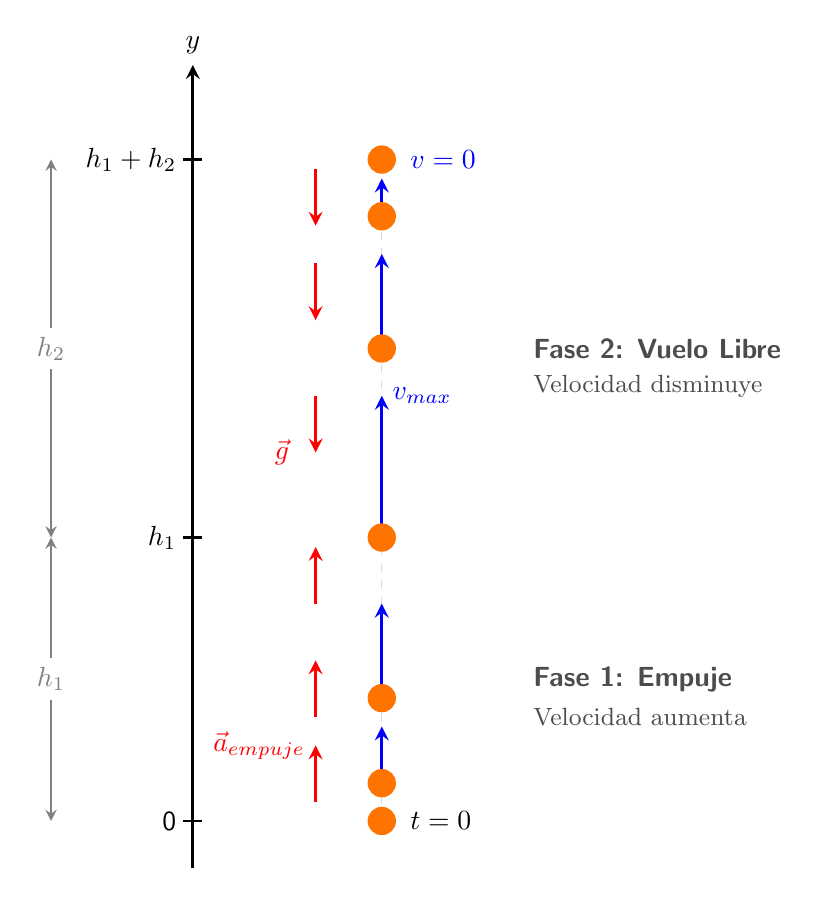
\begin{tikzpicture}[scale=1.2, >=stealth, font=\sffamily]
	
	% ================= EJE Y Y REFERENCIAS =================
	% Eje vertical
	\draw[->, very thick] (0,-0.5) -- (0,8) node[above] {$y$};
	
	% Marcas en el eje
	\draw[thick] (-0.1,0) -- (0.1,0) node[left=0.2cm] {0};
	\draw[thick] (-0.1,3) -- (0.1,3) node[left=0.2cm] {$h_1$};
	\draw[thick] (-0.1,7) -- (0.1,7) node[left=0.2cm] {$h_1+h_2$};
	\node[right] at (2.2, 0) {$t = 0$}; 
	
	% Acotaciones para h1 y h2
	\draw[<->, thick, gray] (-1.5, 0) -- (-1.5, 3) node[midway, fill=white] {$h_1$};
	\draw[<->, thick, gray] (-1.5, 3) -- (-1.5, 7) node[midway, fill=white] {$h_2$};
	
	% Línea punteada suave para guiar la trayectoria
	\draw[dashed, gray!30] (2,0) -- (2,7);
	
	\draw[->, very thick, blue] (2, 5.0) -- (2, 6.0); 
	\draw[->, very thick, blue] (2, 6.4) -- (2, 6.8); 
	\node[right, text=blue] at (2.2, 7.0) {$v = 0$}; 
	
	\draw[->, very thick, blue] (2, 0.4) -- (2, 1.0); 
	\draw[->, very thick, blue] (2, 1.3) -- (2, 2.3); 
	\draw[->, very thick, blue] (2, 3.0) -- (2, 4.5) node[right] {$v_{max}$}; 
	
	% LEYENDA
	%		\draw[thick, rounded corners, fill=gray!5] (4.5, 6) rectangle (7.5, 7.8);
	%		\node[right, font=\bfseries] at (4.6, 7.5) {Leyenda:};
	%		\fill[orange!90!red] (4.8, 7.0) circle (0.12) node[right=0.2cm, black] {Posición};
	%		\draw[->, very thick, blue] (4.8, 6.6) -- (5.6, 6.6) node[right, black] {Velocidad ($\vec{v}$)};
	%		\draw[->, very thick, red] (4.8, 6.2) -- (5.6, 6.2) node[right, black] {Aceleración ($\vec{a}$)};
	
	
	
	% ================= FASE 1: EMPUJE =================
	\node[right, text=black!70] at (3.5, 1.5) {\textbf{Fase 1: Empuje}};
	\node[right, text=black!70, font=\small] at (3.5, 1.1) {Velocidad aumenta};
	
	% Posiciones (distancia decreciente) y Velocidades (flechas decrecientes)
	% El punto t=3 (h1) ya está dibujado
	% t = 4
	\fill[orange!90!red] (2, 5.0) circle (0.15);
	% t = 5
	\fill[orange!90!red] (2, 6.4) circle (0.15);
	% t = 6 (Altura máxima)
	\fill[orange!90!red] (2, 7.0) circle (0.15);
	
	
	
	% Posiciones (distancia creciente) y Velocidades (flechas crecientes)
	% t = 0
	\fill[orange!90!red] (2, 0) circle (0.15); 
	% t = 1
	\fill[orange!90!red] (2, 0.4) circle (0.15);
	% t = 2
	\fill[orange!90!red] (2, 1.3) circle (0.15);
	% t = 3 (Punto de soltar h1)
	\fill[orange!90!red] (2, 3.0) circle (0.15);
	
	
	% Aceleración de empuje (Hacia arriba, constante)
	\draw[->, very thick, red] (1.3, 0.2) -- (1.3, 0.8) node[left] {$\vec{a}_{\text{empuje}}$};
	\draw[->, very thick, red] (1.3, 1.1) -- (1.3, 1.7);
	\draw[->, very thick, red] (1.3, 2.3) -- (1.3, 2.9);
	
	% ================= FASE 2: VUELO LIBRE =================
	\node[right, text=black!70] at (3.5, 5.0) {\textbf{Fase 2: Vuelo Libre}};
	\node[right, text=black!70, font=\small] at (3.5, 4.6) {Velocidad disminuye};
	
	% Aceleración de gravedad (Hacia abajo, constante)
	\draw[->, very thick, red] (1.3, 4.5) -- (1.3, 3.9) node[left=0.2cm] {$\vec{g}$};
	\draw[->, very thick, red] (1.3, 5.9) -- (1.3, 5.3);
	\draw[->, very thick, red] (1.3, 6.9) -- (1.3, 6.3);
\end{tikzpicture}




% FIGURA 2 ------------------------------------------------------------------------------------------------------------
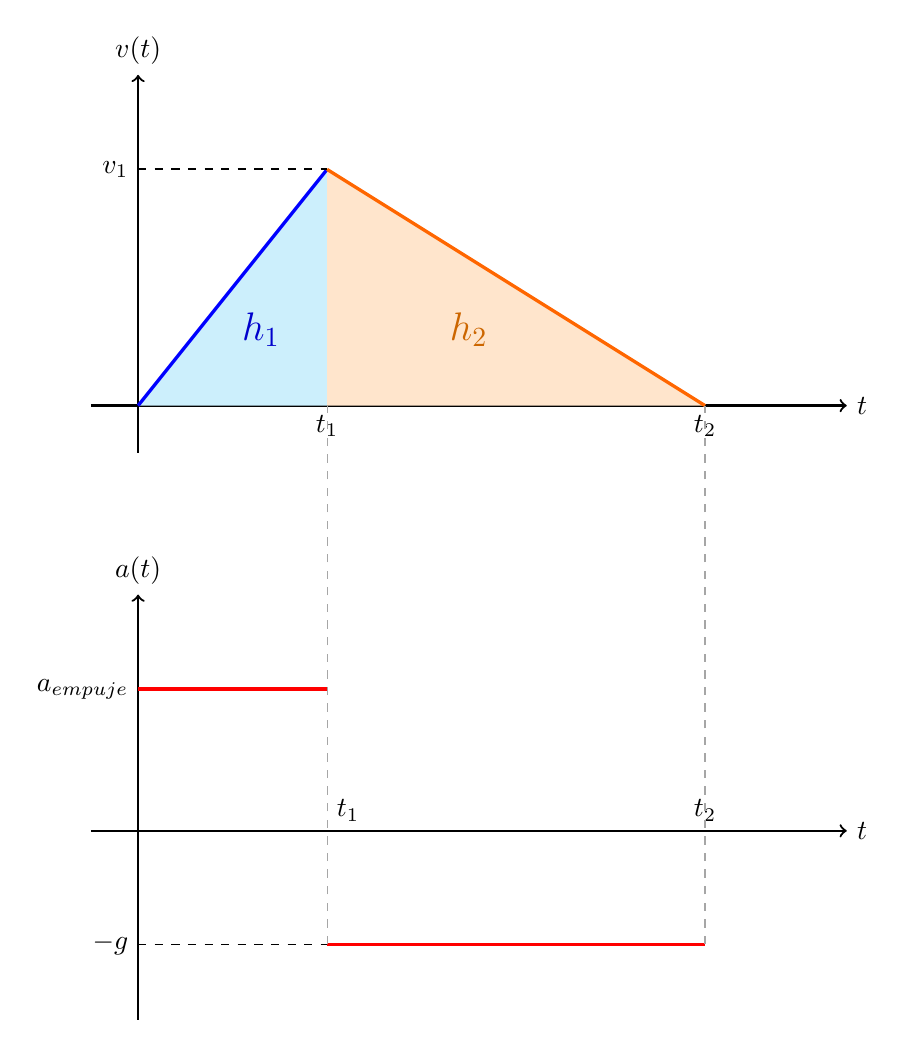
\begin{tikzpicture}[scale=1.2, font=\sffamily]
	
	% ================= GRÁFICO DE VELOCIDAD =================
	\begin{scope}[yshift=4.5cm] % Desplazamiento hacia arriba
		% Ejes
		\draw[->, thick] (-0.5, 0) -- (7.5, 0) node[right] {$t$};
		\draw[->, thick] (0, -0.5) -- (0, 3.5) node[above] {$v(t)$};
		
		% Áreas sombreadas (h1 y h2)
		\fill[cyan!20] (0,0) -- (2,2.5) -- (2,0) -- cycle;
		\fill[orange!20] (2,0) -- (2,2.5) -- (6,0) -- cycle;
		
		% Líneas de la función
		\draw[very thick, blue] (0,0) -- (2,2.5);
		\draw[very thick, orange!80!red] (2,2.5) -- (6,0);
		
		% Líneas punteadas de referencia
		\draw[dashed, thick] (0, 2.5) -- (2, 2.5);
		
		% Textos y Etiquetas
		\node[left] at (0, 2.5) {$v_1$};
		\node[below] at (2, 0) {$t_1$};
		\node[below] at (6, 0) {$t_2$};
		
		% Etiquetas de las áreas
		\node[text=blue!80!black] at (1.3, 0.8) {\Large $h_1$};
		\node[text=orange!80!black] at (3.5, 0.8) {\Large $h_2$};
		
		% Título
		%			\node[above] at (3.5, 3.5) {\textbf{Gráfico de Velocidad vs. Tiempo}};
	\end{scope}
	
	% ================= GRÁFICO DE ACELERACIÓN =================
	\begin{scope}[yshift=0cm]
		% Ejes
		\draw[->, thick] (-0.5, 0) -- (7.5, 0) node[right] {$t$};
		\draw[->, thick] (0, -2) -- (0, 2.5) node[above] {$a(t)$};
		
		% Líneas de la función (Aceleración constante a_empuje y luego -g)
		\draw[very thick, red] (0, 1.5) -- (2, 1.5);
		\draw[very thick, red] (2, -1.2) -- (6, -1.2);
		
		% Salto o discontinuidad
		%			\draw[dashed, red, thick] (2, 1.5) -- (2, -1.2);
		
		% Líneas punteadas de referencia a los ejes
		%			\draw[dashed] (0, 1.5) -- (2, 1.5);
		\draw[dashed] (0, -1.2) -- (2, -1.2);
		
		% Textos y Etiquetas
		\node[left] at (0, 1.5) {$a_{\text{empuje}}$};
		\node[left] at (0, -1.2) {$-g$};
		\node[above right] at (2, 0) {$t_1$};
		\node[above] at (6, 0) {$t_2$};
		
		% Título
		%			\node[above] at (3.5, 2.5) {\textbf{Gráfico de Aceleración vs. Tiempo}};
	\end{scope}
	
	% ================= LÍNEAS DE ALINEACIÓN VERTICAL =================
	% Conectan t1 y t_total a través de ambos gráficos para guiar el ojo
	\draw[dashed, gray!70] (2, -1.2) -- (2, 4.5);
	\draw[dashed, gray!70] (6, -1.2) -- (6, 4.5);
	
\end{tikzpicture}